\section{The Large Hadron Collider}
\label{sec:lhc}

The LHC~\cite{LHCMachine} is a circular particle accelerator, with a 27~kilometer circumference,
located at an average distance of 100 meters beneath the surface of the Earth.
It is nominally used for proton-proton ($pp$) collisions, wherein two counter-rotating
beams of protons are made to collide head-on at specific interaction points (IP) along the 27~kilometer
ring, but can also be run in heavy-ion configurations wherein proton-lead ($p$-Pb) or lead-lead (Pb-Pb)
collisions take place.\footnote{The specific lead (Pb) species used in collisions is $^{208}_{82}$Pb.}\footnote{More rarely, the LHC can also be used to circulate gold (Au) ions.
There are even plans to have proton-oxygen ($p$-O) runs in the future, which will allow
for the LHC experiments to provide research that potentially complements dark matter research
based on cosmic-ray air showers.}
{\color{red}{Multi-year runs of the LHC, in which protons are circulating are referred to as `Runs'. There have been
two so far, Run-I and Run-II,... See Table... --- perhaps describe this or put table after lumi discussion?}}
The $pp$ collisions take priority over those of the heavy-ions, with the collisions each year
consisting of only a few weeks in the winter for the heavy-ion configurations and typically
six to seven months for the $pp$ configuration. The LHC is designed to accelerate protons to a
center-of-mass energy of $\sqrt{s} = 14\,\TeV$.

\subsection{Machine Design and Layout}
\label{sec:lhc_layout}

\paragraph{Machine Composition} \mbox{} \\
\label{sec:dipole}
The LHC was planned as the successor to the Large Electron Positron (LEP) collider~\cite{LEPI,LEPII}, which was in operation
between the years of 1989 to 2000. LEP is still the most powerful lepton collider to date, having maximal electron-positron
center-of-mass collision energies of 209\,\GeV.
After LEP, the particle physics community knew that the next collider at CERN needed to have $\mathcal{O}(10)$\,\TeV~collision
energies; either to be able to probe from all angles any new physics discovered at LEP and/or the Tevatron~\cite{TevatronDesignI}, or
to provide the necessary power to search for still-elusive hints of BSM physics. At the very least,
given a non-discovery of the Higgs boson at LEP and the Tevatron, the community would need a discovery machine powerful enough
to produce electroweak-scale Higgs bosons and an $\mathcal{O}(10)$ \TeV~hadron collider --- as we now know --- is sufficient for this job.


In order to increase center-of-mass collisions energies, collider designs can take two routes: they can
either increase in size, that is, have larger circumferences (radii), or they can increase the strength of the magnetic
fields used to keep the circulating charged particles in orbit. This can be seen by first considering the expression
for the relativistic cyclotron frequency, $\omega$, of a particle moving in a circular orbit,
\begin{align}
    \omega = \frac{qB}{\gamma m},
    \label{eq:rel_cyclotron}
\end{align}
where $m$ is the particle's rest mass, $B$ is the magnitude of the magnetic field experienced by the
particle, $q$ is the particle's electric charge, and $\gamma$ is the relativistic Lorentz factor, $\gamma = \sqrt{1 - \beta^2} = \sqrt{1 - (v/c)^2}$,
with $v$ the particle's velocity and $c$ the speed of light.
Using Eqn.~\ref{eq:rel_cyclotron}, it can be seen that a particle of higher energy confined to a fixed
circular orbit necessarily has a higher angular velocity by relating the particle's angular
velocity to its kinetic energy:
%A particle of higher energy confined
%to a fixed circular orbit necessarily has a higher
%angular velocity, which can be seen by the expression relating the above angular velocity of the particle to its kinetic energy:
\begin{align}
    E_{\text{kin}} \propto m v^2 = m(\omega R)^2 = \frac{q^2 B^2 R^2}{m \gamma^2}.
    \label{eq:kinetic_energy_gen}
\end{align}
In planning the construction of the LHC, the costs in civil engineering and real-estate works that would
be required to construct a larger tunnel in which to house the LHC ring (increasing $R$) far outweighed
the costs of research into and development of magnet systems strong enough to bend the
multi-\TeV~particles along the beam orbit prescribed by the already-existing LEP tunnel (increasing $B$).
The desired center-of-mass collision energy of $\mathcal{O}(10)$\,\TeV, the fact that the LHC would be a hadron (proton)
collider, and the fact that the LHC would be using the existing LEP tunnel dictate the required magnetic
field strength needed to keep the protons in stable orbits at the LHC. This
is seen by using Eqn.~\ref{eq:kinetic_energy_gen}, solving for $B$, and comparing the LHC and LEP
design parameters,
\begin{align}
    \hspace{-0.4cm}
    \frac{B^2_{\text{LHC}}}{B^2_\text{LEP}} &= \frac{ (E_{\text{LHC}} m_{\text{LHC}} \gamma_{\text{LHC}}^2) / (q_{\text{LHC}}^2 R_{\text{LHC}}^2)  } { (E_{\text{LEP}} m_{\text{LEP}} \gamma_{\text{LEP}}^2) / (q_{\text{LEP}}^2 R_{\text{LEP}}^2) } \label{eq:lhc_mag_field} \\
        &= (E_{\text{LHC}} / E_{\text{LEP}}) \times (m_{\text{LHC}} / m_{\text{LEP}}) \times (\gamma_{\text{LHC}}^2 / \gamma_{\text{LEP}}^2) \times (q_{\text{LEP}}^2 / q_{\text{LHC}}^2) \times (R_{\text{LEP}}^2 / R_{\text{LHC}}^2) \notag \\
        &\approx ( 1\,\TeV~/0.2\,\TeV) \times (m_p/ m_e) \times (1) \times (1) \times (1) \notag \\
        &\approx 10^4 \notag,
\end{align}
which shows that the strength of the LHC bending magnets must be on the order of $100\times$
the strength of those used at LEP. The magnetic fields experienced by the electron and positron beams
at LEP were 0.22 Tesla. By Eqn.~\ref{eq:lhc_mag_field}, the LHC bending magnets should achieve magnetic field
strengths on the order of 10 Tesla in order to achieve the desired collision energies.
The maximum achievable magnetic field of conventional ferrormagnets is about 2 Tesla.
To meet the $\sqrt{s}\approx$10\,\TeV~design goal, the magnet system used by the LHC to confine the protons to their circular orbits
must then be composed of \textit{superconducting} electromagnets. %\footnote{Note that even though
%the main dipole bending magnets at LEP were not superconducting, its focusing quadrupole magnets
%\textit{were} superconducting. There are simply fewer quadrupole magnets, as compared to the number of
%dipole magnets, required for a particle collider.}
The entire magnet system of LEP was therefore removed and replaced with superconducting
niobium-titanium (Nb-Ti) alloy based electromagnets which are superconducting
at temperatures below $10$\,K.
%All of the magnets at the LHC are constructed with
%current carrying elements composed of a niobium-titanium (Nb-Ti) alloy that becomes superconducting
%for temperatures below $10$\,K.
To reach temperatures below this $10$\,K threshold, the LHC magnets
are housed in cryostats that allow for the Nb-Ti elements to be fully submerged in a bath
of superfluid Helium at a temperature of $1.9$\,K~\cite{Casas:1992nf}.
In total, the LHC contains more than 120 tonnes of superfluid Helium.
It goes without saying that there is a significant amount of resources and person power at CERN devoted to the refrigeration and cryogenics
systems that are required for the LHC to run.

Additionally, the fact that LEP was a \textit{particle-antiparticle} collider meant that the counter-rotating
beams could be made to occupy a single ring: the same magnetic field could produce counter-rotating beams of
electrons and positrons within the same beam pipe.\footnote{The electrons and positrons at LEP were vertically separated
within the beam pipe by electrostatic separators placed throughout the LEP ring. Turning off these separators
is, to first approximation, how the LEP operators would get the electrically-attracting electrons and positrons to collide.}
As a result, the LEP beam tunnel was constructed with only a single ring in mind and is relatively narrow: the LEP tunnel,
and therefore LHC tunnel, is only $\approx$3.7\,m wide on average.
As the LHC is a \textit{particle-particle} collider, it necessarily requires \textit{two} magnetic fields
of opposing polarity to circulate one of its beams in the clockwise direction and the other in the
counter-clockwise direction.
Given the limited space in the tunnel, however, it is not possible to house two separate rings
of superconducting bending magnets with all of the services that they require \textit{in addition} to the requisite
minimal space needed for personnel and maintenence access.
This forced the need of the so-called `2-in-1' design of the main bending magnets of the LHC, wherein the two
beam pipes are housed in the same cryostat in which the counter-rotating beams are held in their
respective orbits by coupled magnetic fields.
An illustration of this now-iconic design of the LHC bending (dipole) magnets and surrounding cryostat and containment structure is illustrated in Figure~\ref{fig:lhc_dipole_xsec}.
Each of the 15\,meter long superconducting dipole electromagnets of the LHC responsible for constraining the protons to their circular
orbits has currents of $11850$\,Amperes flowing through it and achieves magnetic field strengths of $8.33$\,Tesla.

\begin{figure}[!htb]
    \begin{center}
        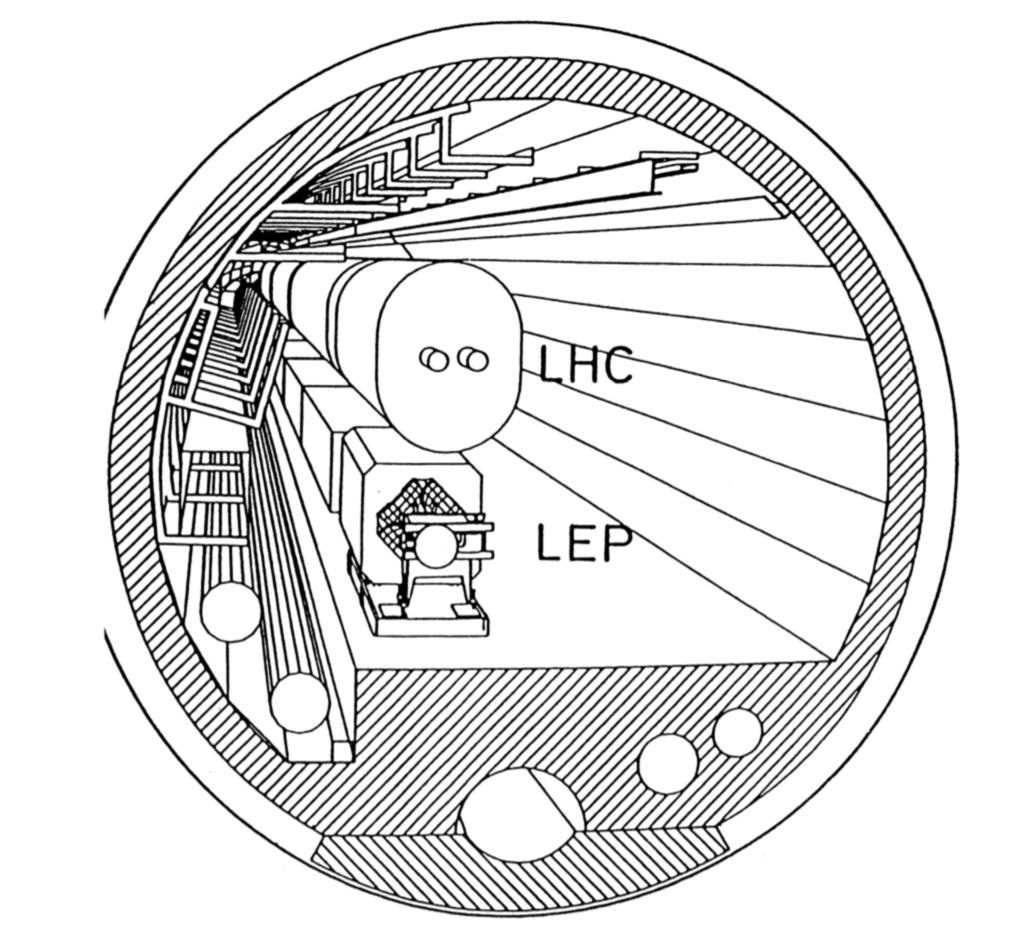
\includegraphics[width=0.43\textwidth]{figures/chapter2/lhc_lep_dipole_comp}
        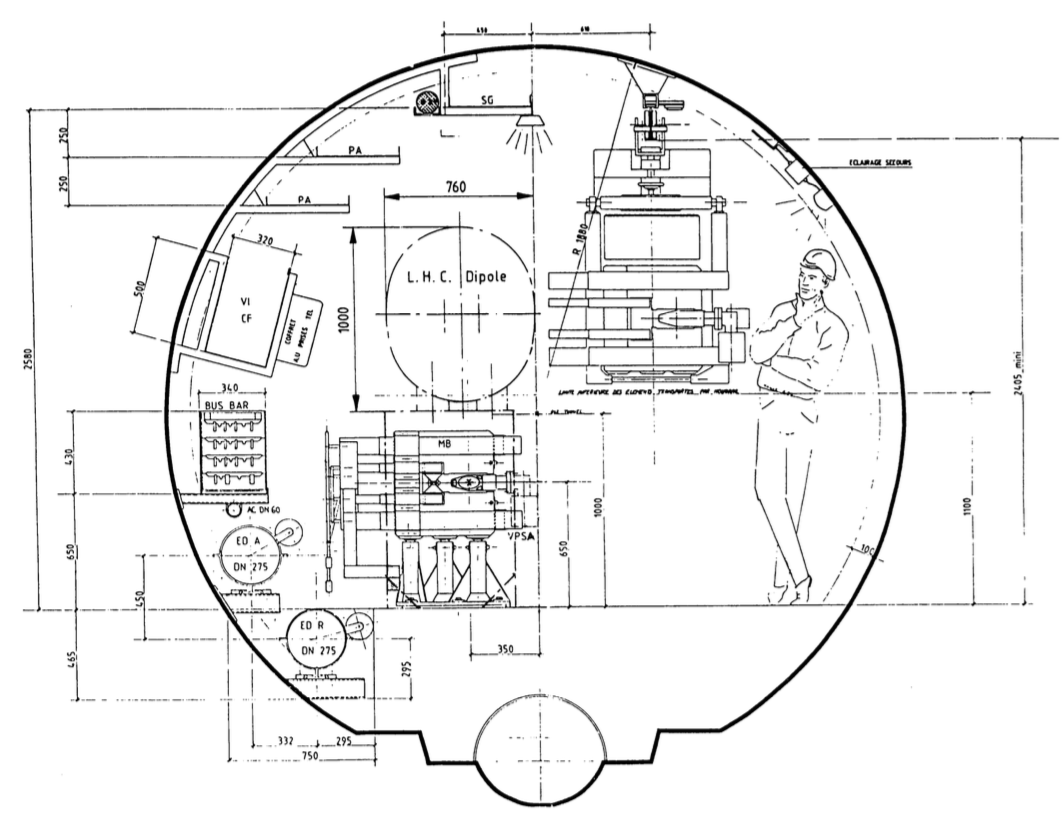
\includegraphics[width=0.50\textwidth]{figures/chapter2/lhc_lep_dipole_comp_person}
        \caption{
            \textit{Left}: Illustration comparing the size of a `2-in-1' LHC dipole configuration to the
                LEP dipole and how they fit inside of the LEP/LHC tunnel. Note that prior to LHC operation,
                the LEP magnets will have been removed: the two are shown side-by-side for comparison purposes only.
            \textit{Right}: Cross-sectional view of the LEP/LHC tunnel with a comparison of the LHC `2-in-1' dipole
                on top of the LEP dipole. An illustration of an average size person is shown
                for scale. Also shown is the service crane in use, to give an idea of the size required
                for potential maintenance access. Clearly, two single-bore, superconducting rings each similar in size
                to the LEP dipole would not fit comfortably in the tunnel. The LHC `2-in-1' design fits
                in nearly the same area as the LEP dipoles while additionally being able to contain both
                particle beams.
                Figures are taken from Ref.~\cite{ECFALHCinLEP}.
        }
        \label{fig:lhc_lep_dipole_comp}
    \end{center}
\end{figure}

\begin{figure}[!htb]
    \begin{center}
        \begin{minipage}{\textwidth}
        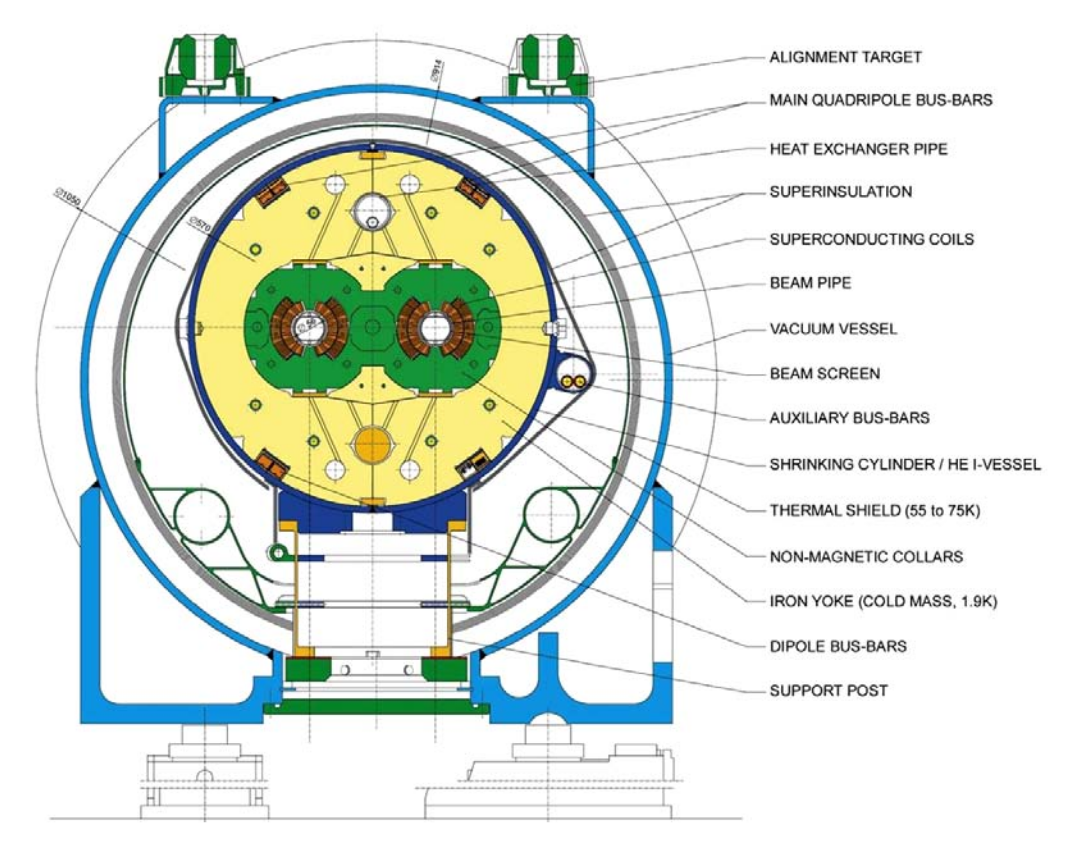
\includegraphics[width=0.59\textwidth]{figures/chapter2/lhc_dipole_fig3p3}
        \raisebox{0.5cm}{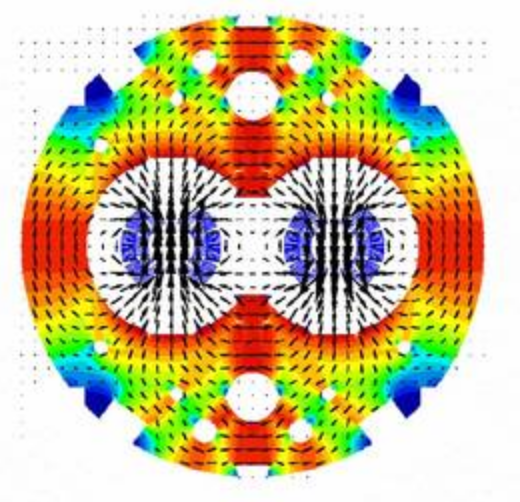
\includegraphics[width=0.4\textwidth]{figures/chapter2/dipole_magnetic_field_lines}}
        \end{minipage}
        \caption{
            \textit{Left}: Cross-sectional view of an LHC dipole bending magnet, with relevant parts indicated.
            The protons orbit inside of the beam pipes, each of which has a diameter of roughly $3$\,cm.
            It is interesting to note that the non-magnetic steel collars (in green) are of critical import
            to the success of the magnet systems. They are required
            to prevent the dipole structure from being deformed or torn apart due to the intense magnetic forces
            tending to push the two beam-pipes apart as a result of their counter-rotating electromagnetic currents.
            These forces amount to about 400 tonnes per meter of dipole when in full operation --- almost equivalent in magnitude
            to the weight of a Boeing 747.
            \textit{Right}: Magnetic field lines of the coupled dipole fields that bend the counter-rotating proton beams
            and keep them in their circular orbits around the LHC ring.
        }
        \label{fig:lhc_dipole_xsec}
    \end{center}
\end{figure}


%\FloatBarrier
\paragraph{Connecting the Dots} \mbox{} \\
The LHC is essentially a chain of superconducting magnets of the type described in the previous paragraphs, where
the the bending (dipole) magnets critical to the LHC design were introduced.
%There are additional
%types of magnets that produce fields of higher multipole moments which, in the case of the quadrupole magnets, are
%necessary for beam \textit{beam focusing}. Conceptually they are very similar to the dipoles and are 
The chain is laid in a double-octagonal structure, illustrated in Figure~\ref{fig:lhc_layout}. There are eight
octants, at the center of which the LHC ring is straight and does not curve.
The LHC curvature occurs at the
boundaries of each of the octants and is primarily made up of bending (dipole) magnets.
The straight sections are where the interaction regions are located and are referred
to as `Points', numbered 1 to 8.
Points 1, 2, 5, and 8 are where the four large LHC experiments are located.
Points 1 and 5 are home to the services and underground areas
of the general purpose experiments, ATLAS and CMS, respectively.
The underground experimental caverns associated with Point 1 and 5 were not present for LEP and
had to be constructed after LEP was retired in 2000.
Figure~\ref{fig:p1} provides an illustration of how the surface and underground
areas are situated at Point 1.
Points 2 and 8 host the services and underground areas of the ALICE and LHCb experiments, respectively.
At these Points, Points 1, 2, 5, and 8, the counter-rotating beams are
made to collide. The remaining Points, Points 3, 4, 6, and 7, are host to various beam `services'
necessary for the operation of the LHC.
Point 3 and 7 host the beam betatron and momentum cleaning (`beam collimation') systems, respectively.
Point 4 hosts the superconducting radio-frequency (RF) systems which accelerate the beams to
their nominal collision energies.
Point 6 is the location of the beam-abort system --- the so-called `beam dump' --- where
the LHC beams may be removed very quickly from the LHC ring by using \textit{kicker} magnets~\cite{LHCDesignI}
that divert the beams out of the LHC ring in a safe manner. The beams may be dumped
if the LHC wishes to refill with protons (or heavy-ions) and needs to remove any
remnants of the previous fill, in case of beam instabilities observed in the LHC ring,
or if one of the experiments signals the need for a beam dump (in case of
beam stability or detector issues observed at the associated IP).

\begin{figure}[!htb]
    \begin{center}
        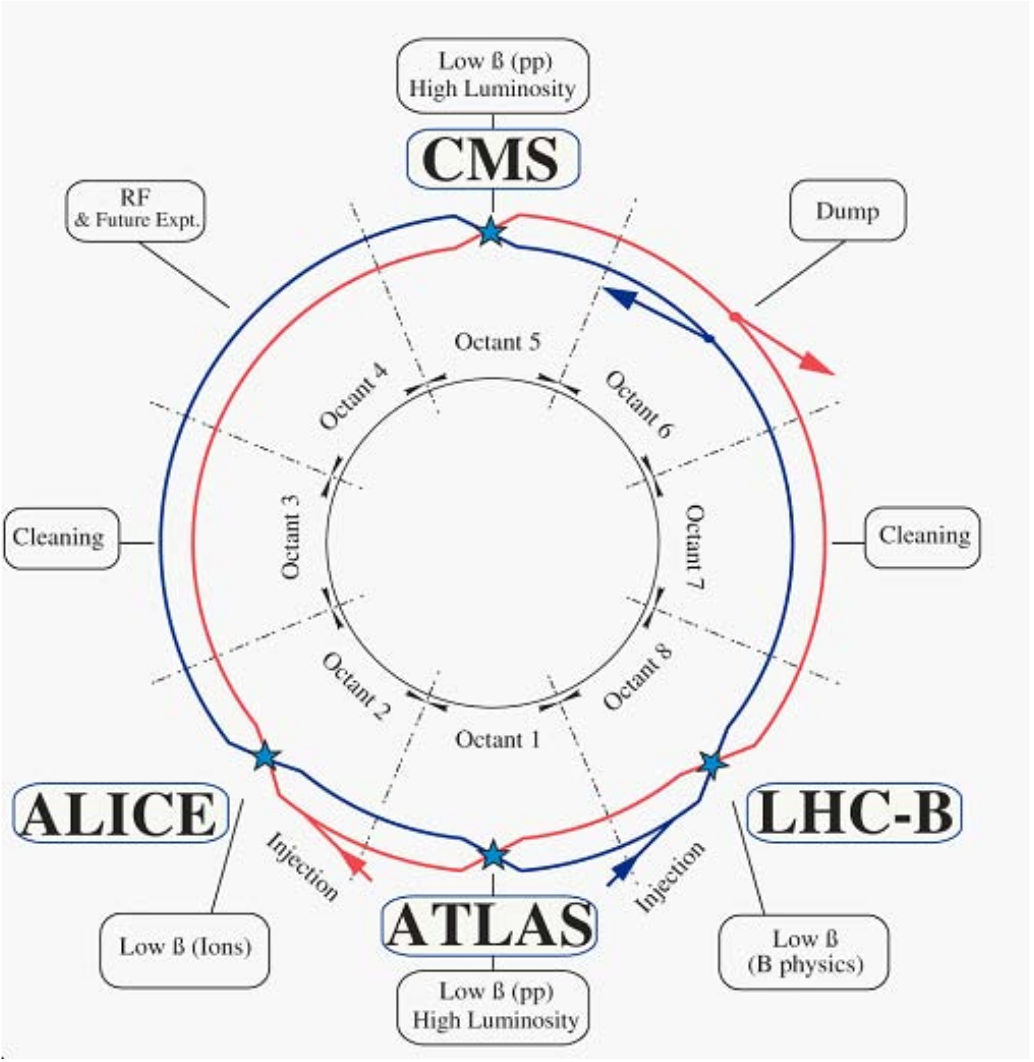
\includegraphics[width=0.8\textwidth]{figures/chapter2/lhc_layout}
        \caption{
            Layout of the LHC and its two counter-rotating beams. Beam 1 is in blue and rotates
            counter-clockwise. Beam 2 is in red and rotates clock-wise.
            At the center of each octant is a straight section which houses
            the experimental caverns or LHC beam facilities.
            At the boundaries of each octant are located the curved sections.
            Figure taken from Figure 2.1 of Ref.~\cite{LHCMachine}.
            {\color{red}{Somewhere $\beta$ should be described -- betatron function}}
        }
        \label{fig:lhc_layout}
    \end{center}
\end{figure}

\begin{figure}[!htb]
    \begin{center}
        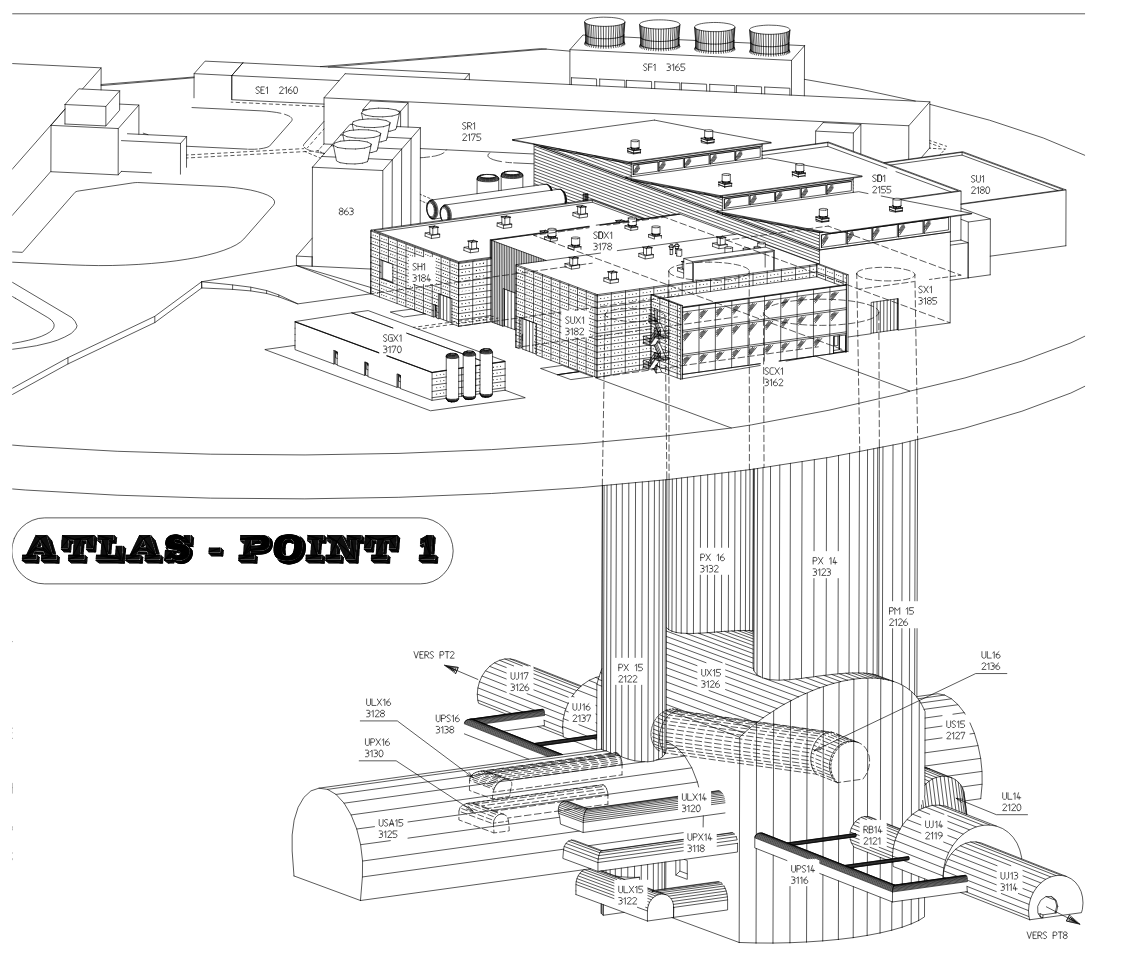
\includegraphics[width=0.75\textwidth]{figures/chapter2/point1_illustration}
        \caption{
            Diagram showing the surface buildings and services and underground areas of Point 1, where
            the ATLAS experiment is located. The LHC ring can be seen at the bottom,
            with its directions indicated by the `VERS PT8 (2)' arrows pointing
            towards Point 8 (2).
            The experimental cavern in which the ATLAS detector sits is UX15.
            The control room for the ATLAS experiment, whereat operators can monitor and
            control the state of the ATLAS detector, is located 100\,m above
            UX15 in the building SCX1.
            Figure taken from Figure 10.1 of Ref.~\cite{LHCDesignII}.
        }
        \label{fig:p1}
    \end{center}
\end{figure}

%\FloatBarrier
\subsection{Injection Chain and Bunch Structure}
\label{sec:lhc_injection}

We now have an idea of how the proton beams relevant to the work
in this thesis are made to circulate in the LHC ring.
In this section we will briefly describe the initial source of the protons and how
they are introduced into the LHC ring.
The LHC relies on a series of pre-acceleration steps that bring the initial
low-energy protons to energies sufficient enough to begin their journey through the LHC.
The sum-total of these steps is referred to as the LHC \textit{injection chain}~\cite{LHCDesignIII}.
The components of the LHC injection chain form the heart of the CERN accelerator
complex illustrated in Figure~\ref{fig:cern_complex}.
For $pp$ collisions in the LHC, the protons are initially sourced from Hydrogen atoms that are released
from a Hydrogen bottle located near Linac 2.
The Hydrogen atoms are immediately stripped of their electrons after passing through
the \textit{duoplasmatron} ion source~\cite{Duoplasma}.
The protons are then passed through Linac 2, a linear accelerator, which accelerates
the protons to $50$\,\MeV.
They then enter the Proton Synchotron Booster (PSB), a circular storage ring
composed of four stacked rings, which accelerates the protons to $1.4\,\GeV$.
The PSB injects the protons into the Proton Synchotron (PS) which accelerates
them to $25$\,\GeV.
The Super Proton Synchotron (SPS) receives the protons from the PS and
accelerates them to $450$\,\GeV.
At this point the protons have sufficient energy to be injected into the LHC.
There are two injection points into the LHC since, up until this stage,
the protons are circulating in the same direction: one injection point sends
protons into the counter-clockwise beamline of the LHC, and the other
into the clockwise beamline.
Until all of the protons from a single \textit{fill} make their way into
the LHC, they will circulate at the injection energy of $450$\,\GeV.
After the filling completes\footnote{A standard LHC fill takes on the order of 4 minutes per
ring.}, the superconducting RF cavities located at Point 4 will begin to accelerate the protons
to their final collision energies.\footnote{If all goes smoothly, this acceleration stage takes roughly 20 minutes.}
The acceleration is achieved by increasing the frequency of the RF oscillations; however,
given that a $450$\,\GeV~proton is already ultra-relativistic, the adjustment of the frequency
needed to get to the collision energies is not large.

The proton beams circulating the LHC are not a continuous stream of protons; rather,
they are grouped into what are referred to as \textit{bunches}.
The protons arrive at the LHC in these bunches which are initially prepared
in the smaller machines that make up the LHC injection chain and then are
kept in their final \textit{bunch structure} by the RF cavities.
The accelerating RF cavities provide an accelerating electromagnetic field
that oscillates longitudinally. The bunches, each composed of roughly $10^{11}$ protons,
are then made to oscillate longitudinally in so-called \textit{synchotron oscillations}
around the central node of the RF oscillation as they circulate through the LHC ring.
The proton bunches are then effectively `shaped' by the oscillating RF field: protons in a bunch
lagging behind or that are ahead of those particles at the center of the bunches
will be accelerated or decelerated accordingly so as to be pushed back into the center of the bunch.
The LHC RF cavities have an oscillation frequency of $400$\,MHz which
defines the boundaries in which proton bunches can lie. These boundaries are
called \textit{RF buckets} and, along with
the circumference of the LHC, dictate the number of proton bunches that
can potentially fit in the LHC.
The relationship between the RF oscillations and the RF bucket and bunch structure
is illustrated in Figure~\ref{fig:lhc_bunch}.
In total, approximately 35640 RF buckets exist when the LHC is in operation.
Not all buckets contain proton bunches, however.
In fact, at the time of the writing of the present thesis,
RF buckets filled with proton bunches have a minimal separation of 10 RF buckets, meaning
that following an RF bucket containing a proton bunch there is at least 9 unfilled RF buckets.
This corresponds to a minimal
time between proton bunches --- the \textit{bunch spacing} --- of $25$\,nanoseconds.
At the time of the present thesis, the operating conditions of the LHC maximally
allow for 2808 $25$\,ns-spaced bunches.\footnote{
The number of allowed bunches is significantly lower than the 35640 RF buckets with $25$\,ns
bunch-spacing potentially allow for. This is due, in part, to the non-trivial bunch-structure
typically employed but also in large part to the fact that there is a rather long \textit{abort gap}
in the LHC ring where no filled RF buckets exist.
The abort gap is a number of continuous unfilled RF buckets that allows the ramp up of the kicker
magnets used for the beam dump to occur in the absence of filled buckets.
In this way, the kicker magnet ramp up does not disturb the structure of the circulating proton beams.
Only after this ramp up is finished should the kicker magnets disturb the beams.
}
The bunch-spacing and overall bunch structure of an LHC fill is not only decided
by the operators of the LHC but also by what the detectors at Points 1,2,5, and 8
can tolerate. This is because shorter bunch spacing means higher intensity and multiplicity
of collisions occuring at each of these IP. A $25$\,nanosecond bunch spacing
corresponds to a maximal $pp$ collision rate of $40$\,MHz. The detectors at each
of the IP have been designed with this collision rate in mind and anything
higher may push them beyond their design limits.

\begin{figure}[!htb]
    \begin{center}
        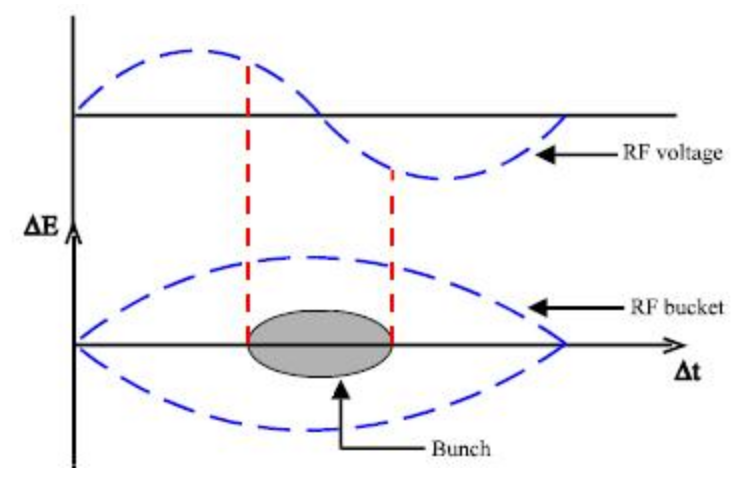
\includegraphics[width=0.5\textwidth]{figures/chapter2/lhc_bunch}
        \caption{
            Illustration of the particle bunch structure in a particle collider such as the LHC.
            The particles are accelerated by radio-frequency (RF) oscillations whose
            amplitude is illustrated in the upper plot.
            The RF bucket's boundary, illustrated in the lower plot, is defined by a full period of the RF oscillation
            and the particle bunch formation, depicted in grey, occurs at the central node of the oscillation.
            The area occupied by the particle bunch is related to the beam's longitudinal
            \textit{emittance}.
        }
        \label{fig:lhc_bunch}
    \end{center}
\end{figure}

\subsection{The Concept of Luminosity}
\label{sec:lhc_luminosity}

In designing a particle collider, the collision energy is not the only important parameter.
Equally important is the value of the instantaneous \textit{luminosity}
that can be achieved by the collider.
An expression for the instantaneous luminosity, $\mathcal{L}$, is given by,
\begin{align}
    \mathcal{L} = \frac{N^2 n_b f}{4 \pi \sigma_x \sigma_y} \cdot S,
    \label{eq:luminosity}
\end{align}
where $N$ is the number of particles per bunch, $n_b$ is the number of colliding bunches,
$f$ is the bunch revolution frequency, $\sigma_{x,y}$ are the transverse beam widths in the
Gaussian approximation, and $S$ is a reduction factor that accounts for geometric factors
such as the non-zero crossing-angle of the colliding beams~\cite{LHCDesignIII,LumiConcept}.
The instantaneous luminosity, $\mathcal{L}$, can be seen by Eqn.~\ref{eq:luminosity}
to have units of cm$^{-2}$s$^{-1}$ and can be conceptually thought of as the
outgoing flux of particles per unit area and time after a bunch crossing in which successful $pp$
collisions occur.
The LHC is designed to deliver collisions to the high luminosity IP (Fig.~\ref{fig:lhc_layout})
at $\mathcal{L} = 10^{34}$\,cm$^{-2}$s$^{-1}$.
Accurate knowledge of $\mathcal{L}$ is of the utmost importance for collider design and operation.
Not only does it parametrise the potential collision rate once the collider beam and bunch
structure are decided, but it allows for the accurate prediction of the number
of collision events, $N_{\text{proc}}$, associated with a particular physics process
with cross-section $\sigma_{\text{proc}}$,
\begin{align}
    N_{\text{proc}} = \sigma_{\text{proc}} \int \mathcal{L}\, \mathrm{d}t \equiv \sigma_{\text{proc}} \cdot L,
    \label{eq:n_exp_lumi}
\end{align}
where $L$ is referred to as the \textit{integrated luminosity} and has units of cm$^{-2}$.
A common unit for integrated luminosity is the \textit{barn}, with symbol `b': one barn is defined as $10^{-24}$\,cm$^{-2}$.
The datasets collected by the LHC experiments are such that the \textit{femtobarn} (fb), $10^{-39}$\,cm$^{-2}$, is relevant.

\subsection{Operation of the Large Hadron Collider}
\label{sec:lhc_operation}

The LHC has been in stable operation since 2009.
It operates in so-called \textit{runs}: multi-year periods of roughly continuous
data-taking.
As CERN shuts down during the winter months, each run is segmented each year
with a several month long shutdown in the winter with a ramp-up period in the spring.
During these shorter shutdowns, maintenance and upgrades may also take place.
In between a given run there is a multi-year break, a \textit{long shutdown},
in which large(er)-scale maintenance and upgrades of both the LHC and the experiments can take place.
At the time of writing, there has so far been two runs of the LHC, Run-I and Run-II.
Run-I took place during the years 2009--2012 and Run-II during 2015--2018.
The integrated luminosities for each of the data taking years between Run-I and Run-II
is shown in Fig.~\ref{fig:int_lumi_multiyear}.
The data relevant to the work presented in this thesis were collected in both
Run-I and Run-II of the LHC, specifically that data collected in the years 2012--2018.
The luminosities (instantaneous and integrated) for these data-taking periods are
shown in Table~\ref{tab:lumi_tab}.
Also shown in Table~\ref{tab:lumi_tab} are the average values of the mean number of interactions per bunch
crossing, $\langle \mu \rangle$, observed during each data-taking year. The quantity $\langle \mu \rangle$
is related to the amount of \textit{pileup} observed during data-taking. Pileup is caused
by overlapping $pp$ interactions within the same (\textit{in-time} pileup) or neighboring (\textit{out-of-time} pileup)
bunch-crossing(s) at the interaction point. The pileup scales with the instantaneous luminosity.
Distributions of $\langle \mu \rangle$ are shown in Fig.~\ref{fig:int_lumi_multiyear} for
the Run-II data-taking period.


\begin{table}[!htb]
    \begin{center}
        \begin{tabular}{l | c | c c c c }
        \hline
        \hline
        & \textbf{Run-I} & \multicolumn{4}{c}{\textbf{Run-II}} \\
        \hline
        Year & 2012 & 2015 & 2016 & 2017 & 2018 \\
        \hline
        Peak Luminosity, $\mathcal{L}$ [cm$^{-2}$s$^{-1}$] ($\times10^{34}$) & $0.77$ & $0.5$ & $1.4$ & $2.1$ & $2.1$ \\ 
        Integrated Luminosity, $L$ [fb$^{-1}$] & 20.2 & 3.2 & 33.0 & 44.3 & 59.9 \\
        Mean number of of interactions & & & & & \\
        \hspace{1.7cm} per bunch crossing, $\langle \mu \rangle$ & 20.7 & 13.4 & 25.1 & 37.8 & 36.1 \\
        \hline
        \hline
        \end{tabular}
        \caption{
        }
        \label{tab:lumi_tab}
    \end{center}
\end{table}

\begin{figure}[!htb]
    \begin{center}
        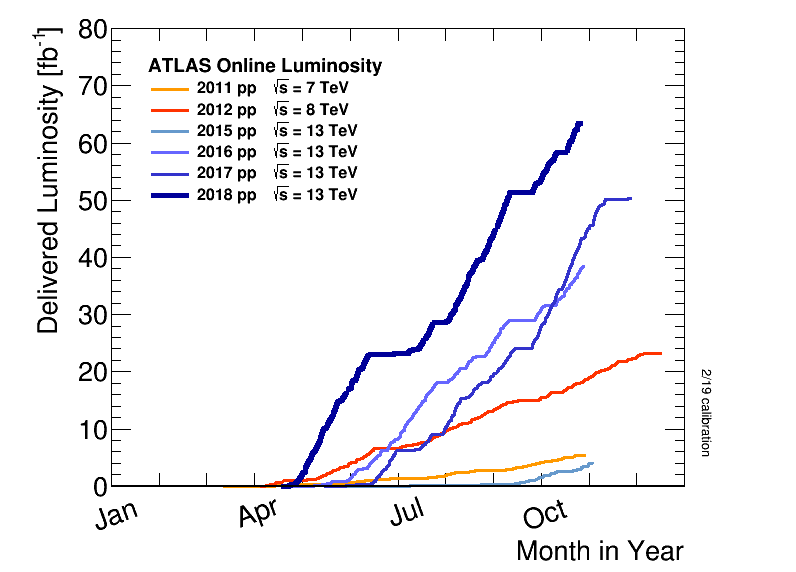
\includegraphics[width=0.49\textwidth]{figures/chapter2/int_lumi_multiyear}
        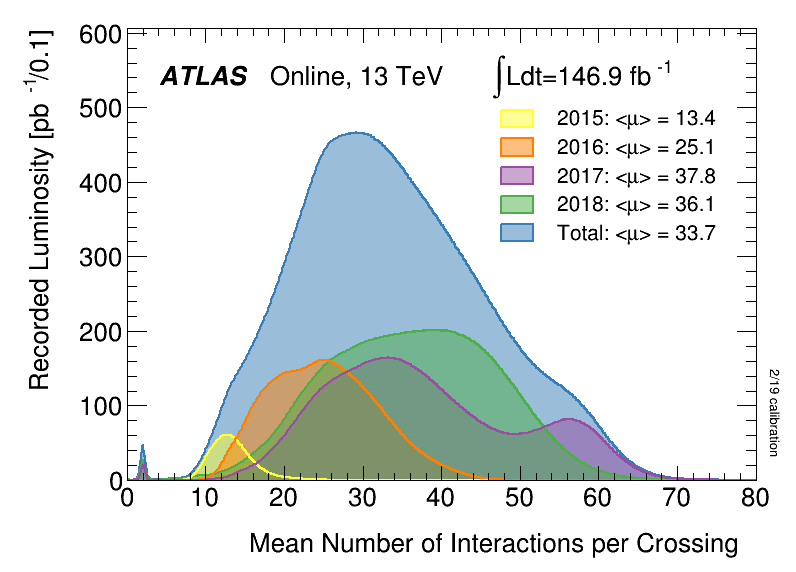
\includegraphics[width=0.49\textwidth]{figures/chapter2/mu_run2}
        \caption{
            \textit{Left}: The ATLAS integrated luminosity during the data-taking years 2011--2018.
            \textit{Right}: The observed average number of $pp$ interactions per bunch-crossing, $\langle \mu \rangle$,
                observed by ATLAS during the Run-II data-taking years, 2015--2018.
        }
        \label{fig:int_lumi_multiyear}
    \end{center}
\end{figure}
